\documentclass[10pt]{report}

\usepackage{amsmath}
\usepackage{amssymb}
\usepackage{graphicx}
\usepackage{helvet}

\setlength{\paperheight}{3in}
\setlength{\paperwidth}{4in}
\pdfpagewidth=\paperwidth
\pdfpageheight=\paperheight

\setlength{\textwidth}{3.5in}
\setlength{\textheight}{2.5in}

\setlength{\oddsidemargin}{-0.75in}
\setlength{\evensidemargin}{-0.75in}
\setlength{\topmargin}{-1.25in}

\newcommand{\sld}[1]{\newpage{\noindent\Large \underline{#1}}\vspace*{8pt}}
\newcommand{\itm}[1]{\vspace*{8pt}\noindent#1}
\newcommand{\itmb}{\itm{$\bullet$}\ }

\newcounter{gmlrx}
\newcounter{gmlry}
\newcommand{\gmnode}[3]{\put(#1,#2){\circle{20}}\put(#1,#2){\makebox(0,0){$#3$}}}
\newcommand{\gmplate}[5]{
\setcounter{gmlrx}{#1}\addtocounter{gmlrx}{#3}
\setcounter{gmlry}{#2}\addtocounter{gmlry}{-#4}
\put(#1,#2){\line(1,0){#3}}
\put(#1,#2){\line(0,-1){#4}}
\put(\value{gmlrx},\value{gmlry}){\line(-1,0){#3}}
\put(\value{gmlrx},\value{gmlry}){\line(0,1){#4}}
\setcounter{gmlrx}{#1}\addtocounter{gmlrx}{5}
\setcounter{gmlry}{#2}\addtocounter{gmlry}{-6}
\put(\value{gmlrx},\value{gmlry}){\makebox(0,0){$#5$}}
}



\begin{document}
\sf%
\vspace*{18pt}
\noindent
{\huge
Hierarchical Models\\[8pt]
of Data Coding
}
\\[24pt]
{\Large Bob Carpenter}
\\[4pt]
(w.\ Emily Jamison and Breck Baldwin)
\\[8pt]
{\large\emph{Alias-i, Inc.}}


\sld{Supervised Machine Learning}

\begin{enumerate}
\item Define coding standard mapping inputs to outputs, e.g.:
\begin{itemize}
\footnotesize
\item English word $\rightarrow$ stem
\item newswire text $\rightarrow$ person name spans
\item biomedical text $\rightarrow$ genes mentioned
\end{itemize}
\item Collect inputs and code ``gold standard'' training data
\item Develop and train statistical model using data
\item Apply to unseen inputs
\end{enumerate}



\sld{Coding Bottleneck}

\begin{itemize}
\item Bottleneck is collecting training corpus
\item Commericial data's expensive (e.g.\ LDA, ELRA)
\item Academic corpora typically restrictively licensed
\item Limited to existing corpora
\item For new problems, use:
self, grad students, temps, interns, \ldots
\vspace*{12pt}
\item Crowdsourcing to the rescue (e.g. Mechanical Turk)
\end{itemize}

\newpage
\vspace*{36pt}
\noindent
{\huge Case Studies}

\vspace*{24pt}
{}\noindent
(Mechanical Turked, but same for ``experts''.)

\sld{Case 1: Named Entities}

\hspace*{-24pt}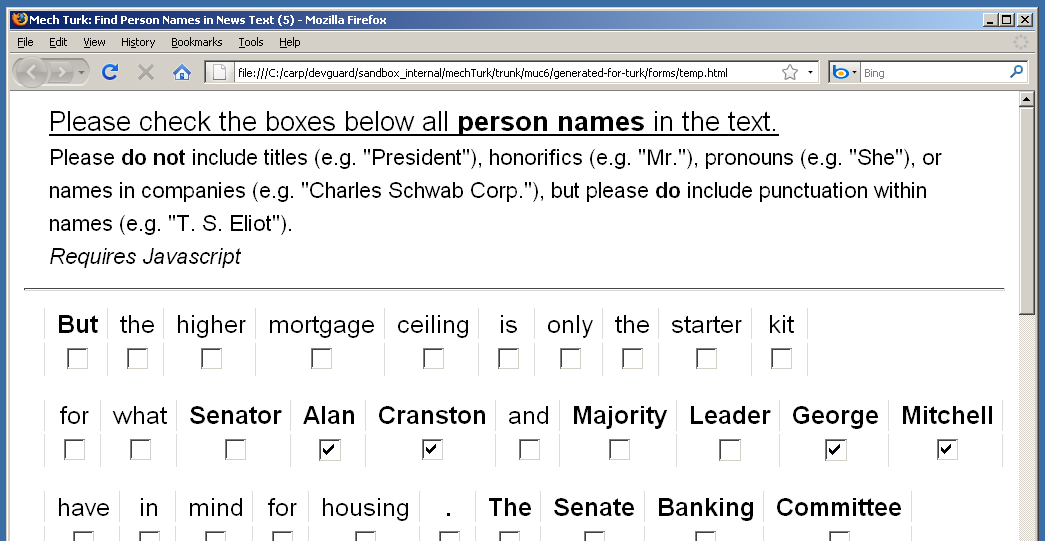
\includegraphics[width=1.05\textwidth]{pngs/big-ne-form.png}


\sld{Named Entities Worked}

\begin{itemize}
\item Conveying the coding standard
\begin{itemize}
\footnotesize
\item official MUC-6 standard dozens of pages
\item examples are key
\item (maybe a qualifying exam)
\end{itemize}

\item User Interface Problem
\begin{itemize}
\footnotesize
\item highlighting with mouse too fiddly (see Fitt's Law)
\item one entity type at a time (vs. pulldown menus)
\item checkboxes (vs. highlighting spans)
\end{itemize}
\end{itemize}

\sld{Discussion: Named Entities}

\vspace*{-6pt}
\begin{itemize}
\item 190K tokens, 64K capitalized, 4K names
\item Less than a week at 2 cents/400 tokens (US\$95)
\item Turkers overall better than LDC data
\begin{itemize}
\footnotesize
\item Correctly Rejected:
{\tt\footnotesize Webster's, Seagram, Du Pont,
\\
Buick-Cadillac, Moon, erstwhile Phineas Foggs}
\item Incorrectly Accepted: {\tt\footnotesize Tass}
\item Missed Punctuation: {\tt\footnotesize J~E.~``Buster'' Brown}
\end{itemize}
\item Many Turkers no better than chance \\
(c.f.\ social psych by Yochai Benkler, Harvard)
\end{itemize}


\sld{Case 2: Morphological Stemming}

\hspace*{-24pt}
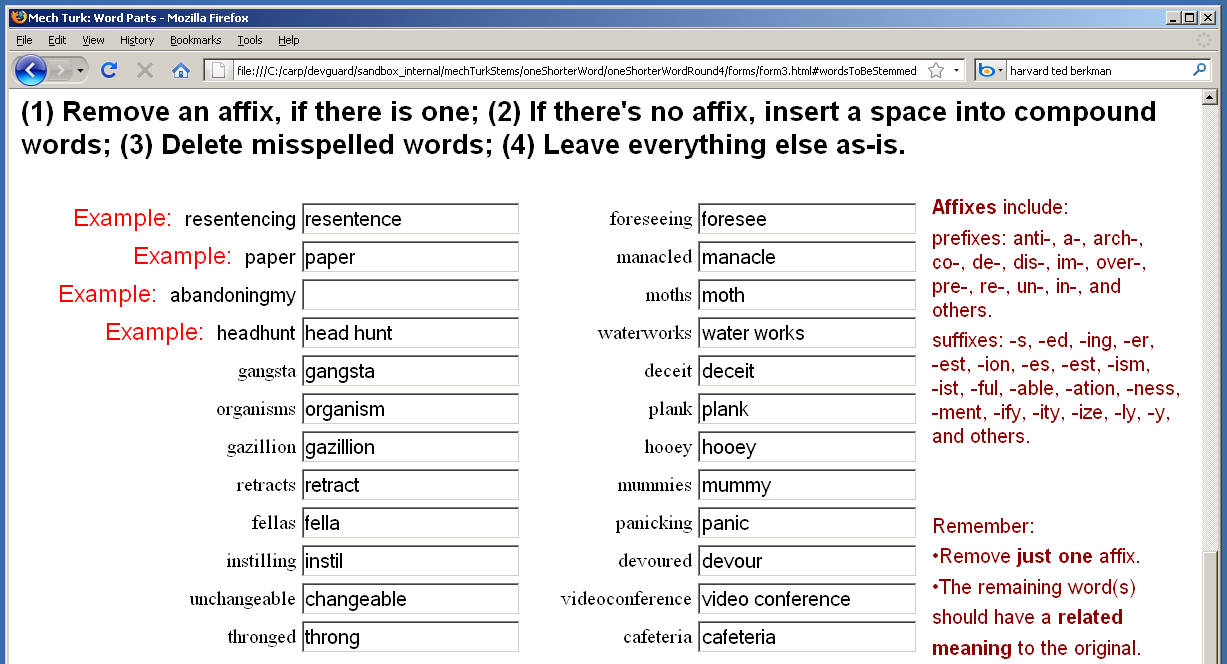
\includegraphics[width=1.05\textwidth]{pngs/stems-v4.png}


\sld{Morphological Stemming Worked}

\begin{itemize}
\vspace*{-8pt}
\item Three iterations on coding standard
\begin{itemize}
\footnotesize
\item simplified task to one stem
\end{itemize}

\item Four iterations on final standard instructions
\vspace*{-6pt}
\begin{itemize}
\footnotesize
\item added previously confusing examples
\end{itemize}

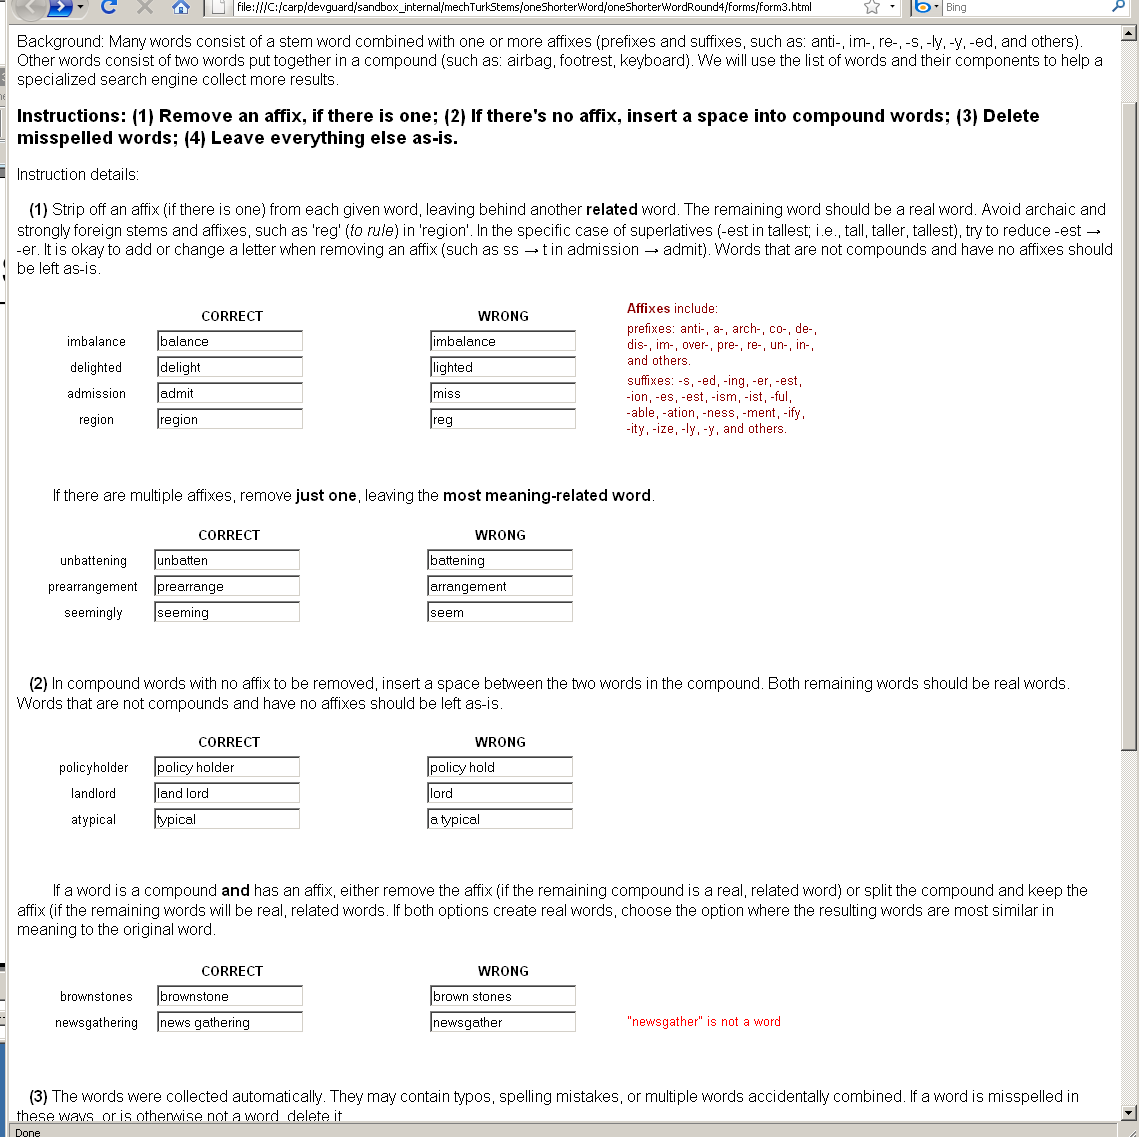
\includegraphics[width=0.2\textwidth]{pngs/stems-instrux.png}

\item Added qualifying test

\end{itemize}



\sld{Case 3: Gene Linkage}

\hspace*{-24pt}
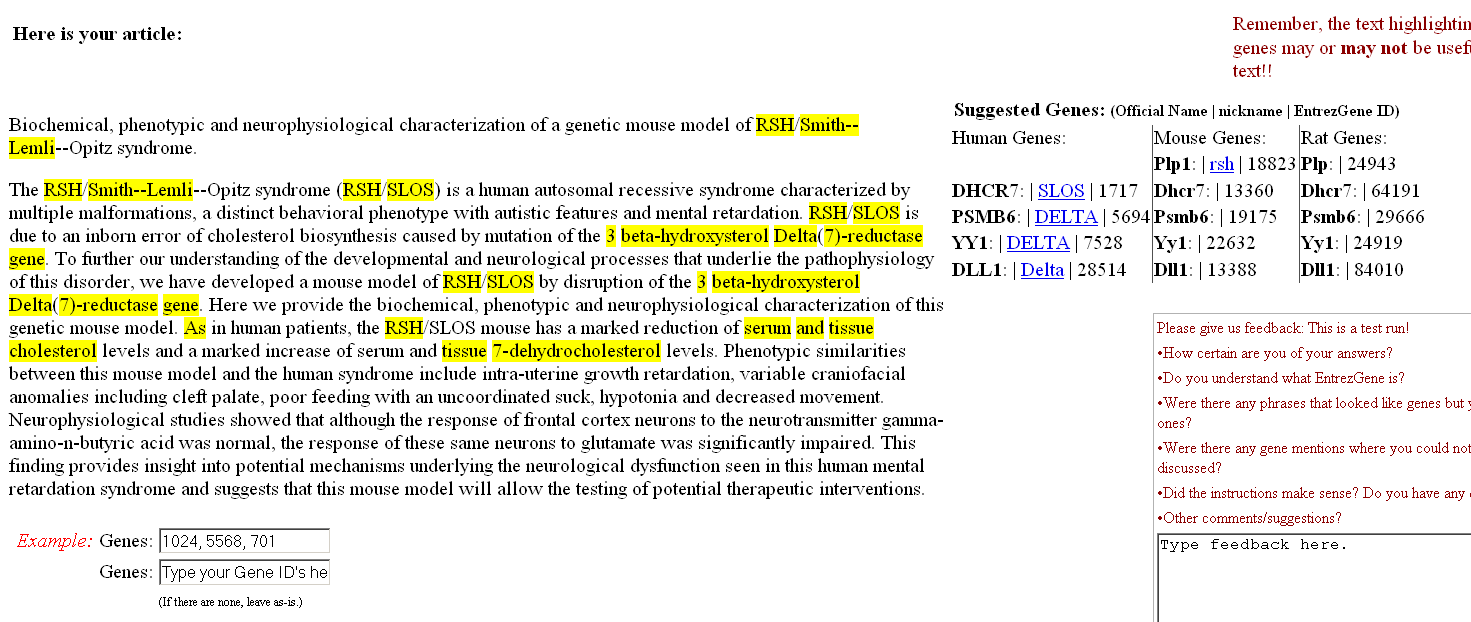
\includegraphics[width=1.05\textwidth]{pngs/gene-task.png}

\sld{Gene Linkage Failed}

\begin{itemize}
\item {\bfseries Could} get Turkers to pass qualifier
\item {\bfseries Could not} get Turkers to take task even at \$1/hit
\item Doing coding ourselves (5-10 minutes/HIT)
\vspace*{12pt}
\item How to get Turkers do these complex tasks?
\begin{itemize}
\footnotesize
\item Low concentration tasks done quickly
\item Compatible with studies of why Turkers Turk
\end{itemize}
\end{itemize}


\newpage
\vspace*{36pt}
\noindent
{\huge {\Huge $\kappa$} Statistics}


\sld{{\Huge $\kappa$} is ``Chance-Adjusted Agreement''}

$\kappa(A,E) = {\displaystyle\frac{A - E}{1 - E}}$



\begin{itemize}
\item $A$ is agreeement rate 
\item $E$ is chance agreement rate
\end{itemize}
\vspace*{8pt}
\begin{itemize}
\item Industry standard
\item Attempts to adjust for difficulty of task
\item $\kappa$ above arbitrary threshold considered ``good''
\end{itemize}

\sld{Problems with {\Huge $\kappa$}}

\begin{itemize}
\item $\kappa$ intrinsically a pairwise measure
\item $\kappa$ only works for subset of shared annotations
\item Not used in inference after calculation
\begin{itemize}
\footnotesize
\item $\kappa$ doesn't predict corpus accuracy 
\item $\kappa$ doesn't predict annotator accuracy 
\end{itemize}
\item $\kappa$ reduces to agreement for hard problems
\begin{itemize}
\item {\large $\lim_{E \rightarrow 0} \kappa(A,E) = A$}
\end{itemize}
\end{itemize}

\sld{Problems with {\Huge $\kappa$} (cont)}

\begin{itemize}
\item $\kappa$ assumes annotators all have same accuracies
\item $\kappa$ assumes annotators are unbiased 
\begin{itemize}
\footnotesize
\item if biased in same way, $\kappa$ artificially high
\end{itemize}
\item $\kappa$ assumes 0/1 items same value
\begin{itemize}
\footnotesize
\item consider low prevalence, high negative agreement (common)
\end{itemize}
\end{itemize}



\newpage
\vspace*{36pt}
\noindent
{\huge Inferring Gold Standards}


\sld{Voted Gold Standard}

\begin{itemize}
\item Turkers vote
\item Label with majority category
\item Censor if no majority
\end{itemize}
\vspace*{12pt}
\begin{itemize}
\item This is also NLP standard
\item Sometimes adjudicated 
\begin{itemize}
\footnotesize
\item  no reason to trust result
\end{itemize}
\end{itemize}


\sld{Some Labeled Data}

\begin{itemize}
\item Seed the data with cases with known labels
\item Use known cases to estimate coder accuracy
\item Vote with adjustment for accuracy
\item Requires relatively large amount of items for
\begin{itemize}
\footnotesize
\item estimating accuracies well
\item liveness for new items
\end{itemize}
\item Gold may not be as pure as requesters think
\item Some preference tasks have no ``right'' answer
\begin{itemize}
\footnotesize
\item e.g. Dolores Labs': Bing vs. Google, Facestat, Colors, ...
\end{itemize}
\end{itemize}


\sld{Estimate Everything}

\begin{itemize}
\item Gold standard labels
\item Coder accuracies
    \begin{itemize}
\footnotesize
      \item sensitivity = TP/(TP+FN) (false negative rate; misses)
      \item specificity = TN/(TN+FP) (false positive rate; false alarms)
\begin{itemize}
      \item unlke precision, but like $\kappa$, uses TN information
\end{itemize}
      \item imbalance indicates bias; high values accuracy
    \end{itemize}
\item Coding standard difficulty
    \begin{itemize}
\footnotesize
        \item average accuracies
        \item variation among coders
    \end{itemize}
\item Item difficulty (important; needs many annotations)
\end{itemize}

\sld{Benefits of (Bayesian) Estimation}

\begin{itemize}
\item More accurate than voting with threshold
\begin{itemize}
\footnotesize
\item largest benefit with few Turkers/item
\item evaluated with known ``gold standard''
\end{itemize}
\item May include gold standard cases (semi-supervised)
\item Full Bayesian posterior inference
\begin{itemize}
\footnotesize
\item probabilistic ``gold standard''
\item compatible with probabilistic learning, esp.\ Bayesian
\item works well for low counts
\item preservers uncertainty for ovedispersed downstream inference
\end{itemize}
\end{itemize}


\sld{Why Task Difficulty for Smoothing?}

\begin{itemize}
\item What's your estimate for:
\begin{itemize}
\footnotesize
\item a baseball player who goes 50 for 200?
\item a market that goes down 9 out of 10 days?
\item a coin that lands heads 3 out of 10 times?
\item ...
\item an annotator who's correct for 10 of 10 items?
\item an annotator who's correct in 171 of 219 items?
\item \ldots
\end{itemize}
\item Hierarchical model inference for accuracy prior
\begin{itemize}
\footnotesize
\item Smooths estimates for coders with few items
\end{itemize}
\end{itemize}


\sld{Is a 24 Karat Gold Standard Possible?}

\begin{itemize}
\item Or is it fool's gold?
\item Some items are marginal given coding standard
\begin{itemize}
\footnotesize
\item `erstwhile Phineas Phoggs' (person?)
\item `the Moon' (location?)
\item stem of `butcher' (`butch'?)
\end{itemize}
\item  Some items are underspecified in text
\begin{itemize}
\footnotesize
\item `New York' (org or loc?)
\item `fragile X' (gene or disease?)
\item `p53' (gene vs.\ protein vs.\ family, which species?)
\item operon or siRNA transcribed region (gene or ?)
\end{itemize}
\end{itemize}

\sld{Traditional Approach to Disagreeement}

\begin{itemize}
\item Traditional approaches either
\begin{itemize}
\footnotesize
\item censor disagreements, or
\item adjudicate disagreements (revise standard).
\end{itemize}
\item Adjudication may not converge
\vspace*{12pt}
\item But, posterior uncertainty can be modeled
\end{itemize}



\sld{Active Learning}

\begin{itemize}
\item Choose most useful items to code next
\item Typically balancing two criteria
\begin{itemize}
\footnotesize
\item high uncertainty
\item high typicality (how to measure?)
\end{itemize}
\item Can get away with fewer coders/item
\item May introduce sampling bias
\item Compare supervision for high certainty items
\begin{itemize}
\footnotesize
\item High precision (for most customers)
\item High recall (defense analysts and biologists)
\end{itemize}
\end{itemize}


\sld{Code-a-Little, Learn-a-Little}

\begin{itemize}
\item Semi-automated coding
\item System suggests labels
\item Coders correct labels
\item Much faster coding
\item But may introduce bias
\vspace*{12pt}
\item Hugely helpful in practice
\end{itemize}



\newpage
\vspace*{36pt}
\noindent
{\huge Statistical Inference Model}


\sld{Strawman Binomial Model}

\begin{itemize}
\item Prevalence $\pi$ : chance of ``positive'' outcome
\item $\theta_{1,j}$ : annotator $j$'s sensitivity
\item $\theta_{0,j}$ : annotator $j$'s specificity
\item Sensitivities, specifities same ($\theta_{1,j} = \theta_{0,j'}$)
\item Maximum likelihood estimation (or hierarchical prior)
\vspace*{4pt}
\item Hypothesis easily rejected by by $\chi^2$
\begin{itemize}
\footnotesize
\item look at marginals (e.g. number of all-1 annotations)
\item overdispersed relative to simple model
\end{itemize}
\end{itemize}

\sld{Beta-Binomial ``Random Effects''}

\begin{picture}(195,145)

\gmnode{57.5}{132.5}{\alpha_0}
\gmnode{97.5}{132.5}{\beta_0}
\gmnode{142.5}{132.5}{\alpha_1}
\gmnode{182.5}{132.5}{\beta_1}
\gmnode{77.5}{92.5}{\theta_{0,j}}
\gmnode{162.5}{92.5}{\theta_{1,j}}
\gmnode{10}{30}{\pi}
\gmnode{55}{30}{c_i}
\gmnode{120}{30}{x_k}

\put(57.5,122.5){\vector(1,-1){19.75}}  % alpha_0 to theta_0_j
\put(97.5,122.5){\vector(-1,-1){19.75}} % beta_0 to theta_0_j
\put(142.5,122.5){\vector(1,-1){19.75}}  % alpha_1 to theta_1_j
\put(182.5,122.5){\vector(-1,-1){19.75}} % beta_1 to theta_1_j
\put(20,30){\vector(1,0){25}}  % \pi to c_i
\put(65,30){\vector(1,0){45}}  % c_i to x_k
\put(77.5,82.5){\vector(1,-1){42.5}}  % theta_0_j to x_k
\put(162.5,82.5){\vector(-1,-1){42.5}}  % theta_1_j to x_k

\gmplate{30}{55}{50}{50}{I}
\gmplate{95}{55}{50}{50}{K}
\gmplate{45}{115}{150}{45}{J}

\end{picture}

\sld{Sampling Notation}

Label $x_k$ by annotator $i_k$ for item $j_k$

\vspace*{-8pt}
{\footnotesize
\begin{eqnarray*}
\pi & \sim & \mathsf{Beta}(1,1)
\\
c_i & \sim & \mathsf{Bernoulli}(\pi)
\\
\theta_{0,j} & \sim & \mathsf{Beta}(\alpha_0,\beta_0)
\\
\theta_{1,j} & \sim & \mathsf{Beta}(\alpha_1,\beta_1)
\\
x_k & \sim & \mathsf{Bernoulli}(c_{i_k} \theta_{1,j_k}
                                        + (1 - c_{i_k}) (1 - \theta_{0,j_k}))
\end{eqnarray*}}
\begin{itemize}
\item  $\mathsf{Beta}(1,1) = \mathsf{Uniform}(0,1)$
\item  Maximum Likelihood:
$\alpha_0 = \alpha_1 = \beta_0 = \beta_1 = 1$
\end{itemize}

\sld{Hierarchical Component}

\begin{itemize}
\item Estimate priors $\alpha$ and $\beta$
\item With diffuse hyperpriors:
{\footnotesize
\begin{eqnarray*}
\alpha_0/(\alpha_0 + \beta_0) & \sim & \mathsf{Beta}(1,1)
\\
\alpha_0 + \beta_0 & \sim & \mathsf{Pareto}(1.5)
\\
\alpha_1/(\alpha_1 + \beta_1) & \sim & \mathsf{Beta}(1,1)
\\
\alpha_1 + \beta_1 & \sim & \mathsf{Pareto}(1.5)
\end{eqnarray*}}
{\footnotesize {\it note}: \ \ $\mathsf{Pareto}(x|1.5) \propto x^{-2.5}$}

\item Infers appropriate smoothing
\item Estimates annotator population parameters
\end{itemize}

\sld{Gibbs Sampling}

\begin{itemize}
\item Estimates full posterior distribution
\begin{itemize}
\item Not just variance, but shape
\item Includes dependencies (covariance)
\end{itemize}
\item Samples $\theta^{(n)}$ support plug-in predictive inference
\[
p(y|y') = \int p(y'|\theta) \ p(\theta|y) \ d\theta
\approx
\frac{1}{N} \sum_{n < N} p(y'|\theta^{(n)})
\]
\item Robust (compared to EM)
\item Requires sampler for conditionals (automated in BUGS)
\end{itemize}


\sld{BUGS Code}

\vspace*{-12pt}
{\tiny
\begin{verbatim}
model {
  pi ~ dbeta(1,1)
  for (i in 1:I) {
    c[i] ~ dbern(pi)
  }
  for (j in 1:J) {
    theta.0[j] ~ dbeta(alpha.0,beta.0) I(.4,.99)
    theta.1[j] ~ dbeta(alpha.1,beta.1) I(.4,.99)
  }
  for (k in 1:K) {
    bern[k] <- c[ii[k]] * theta.1[jj[k]]
             + (1 - c[ii[k]]) * (1 - theta.0[jj[k]])
    xx[k] ~ dbern(bern[k])
  }
  acc.0 ~ dbeta(1,1)
  scale.0 ~ dpar(1.5,1)  I(1,100)
  alpha.0 <- acc.0 * scale.0
  beta.0 <- (1-acc.0) * scale.0
  acc.1 ~ dbeta(1,1)
  scale.1 ~ dpar(1.5,1) I(1,100)
  alpha.1 <- acc.1 * scale.1;
  beta.1 <- (1-acc.1) * scale.1
}
\end{verbatim}
}

\sld{Calling BUGS from R}

\vspace*{-12pt}
{\tiny
\begin{verbatim}
library("R2WinBUGS")

data <- list("I","J","K","xx","ii","jj")

parameters <- c("c", "pi","theta.0","theta.1",
                "alpha.0", "beta.0", "acc.0", "scale.0",
                "alpha.1", "beta.1", "acc.1", "scale.1")

inits <- function() {
  list(pi=runif(1,0.7,0.8),
       c=rbinom(I,1,0.5),
       acc.0 <- runif(1,0.9,0.9),
       scale.0 <- runif(1,5,5),
       acc.1 <- runif(1,0.9,0.9),
       scale.1 <- runif(1,5,5),
       theta.0=runif(J,0.9,0.9),
       theta.1=runif(J,0.9,0.9))  }

anno <- bugs(data, inits, parameters,
             "c:/carp/devguard/sandbox/hierAnno/trunk/R/bugs/beta-binomial-anno.bug",
              n.chains=3, n.iter=500, n.thin=5,
              bugs.directory="c:\\WinBUGS\\WinBUGS14")
\end{verbatim}
}

\newpage
\vspace*{36pt}
\noindent
{\huge Simulated Data}

\sld{Simulation Study}

\begin{itemize}
\item Simulate data (with reasonable model settings)
\item Test sampler's ability to fit
\item Parameters
\begin{itemize}
\footnotesize
\item 20 annotators, 1000 items
\item 50\% missing annotations at random
\item prevalence $\pi = 0.2$
\item specificity prior $(\alpha_0,\beta_0) = (40,8)$ (83\% accurate)
\item sensitivity prior $(\alpha_1,\beta_1) = (20,8)$ (72\% accurate)
\end{itemize}
\end{itemize}

\sld{Simulated Sensitivities / Specificities}

\begin{itemize}
\item Crosshairs at prior mean
\item Realistic simulation compared to (estimated) real data
\end{itemize}

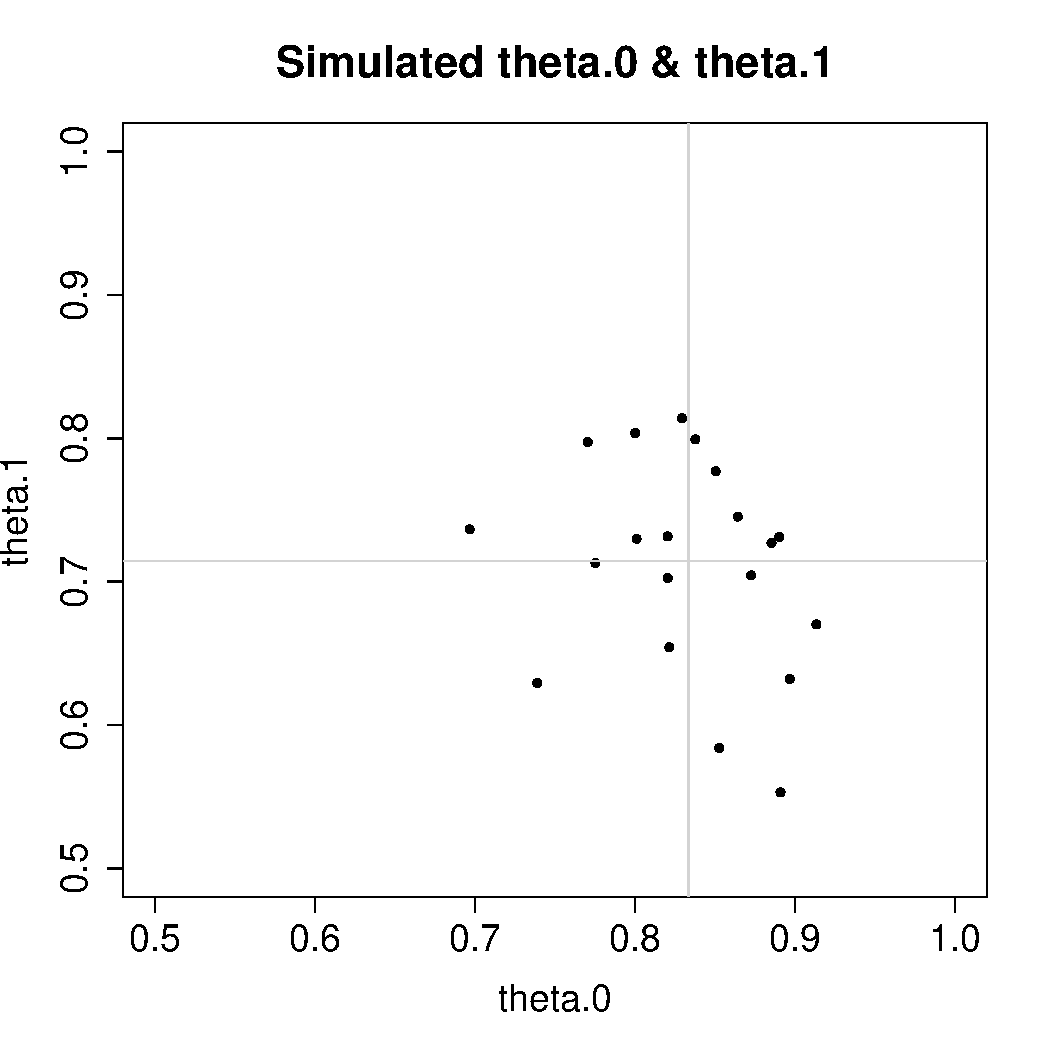
\includegraphics[width=0.4\textwidth]{pdf/beta-binomial-anno-sim-thetas.pdf}%

\sld{Prevalence Estimate}

\begin{itemize}
\item Simulated with $\pi = 0.2$; sample mean $c_i$ was 0.21
\item Estimand of interest in epidemiology (or sentiment)
\end{itemize}

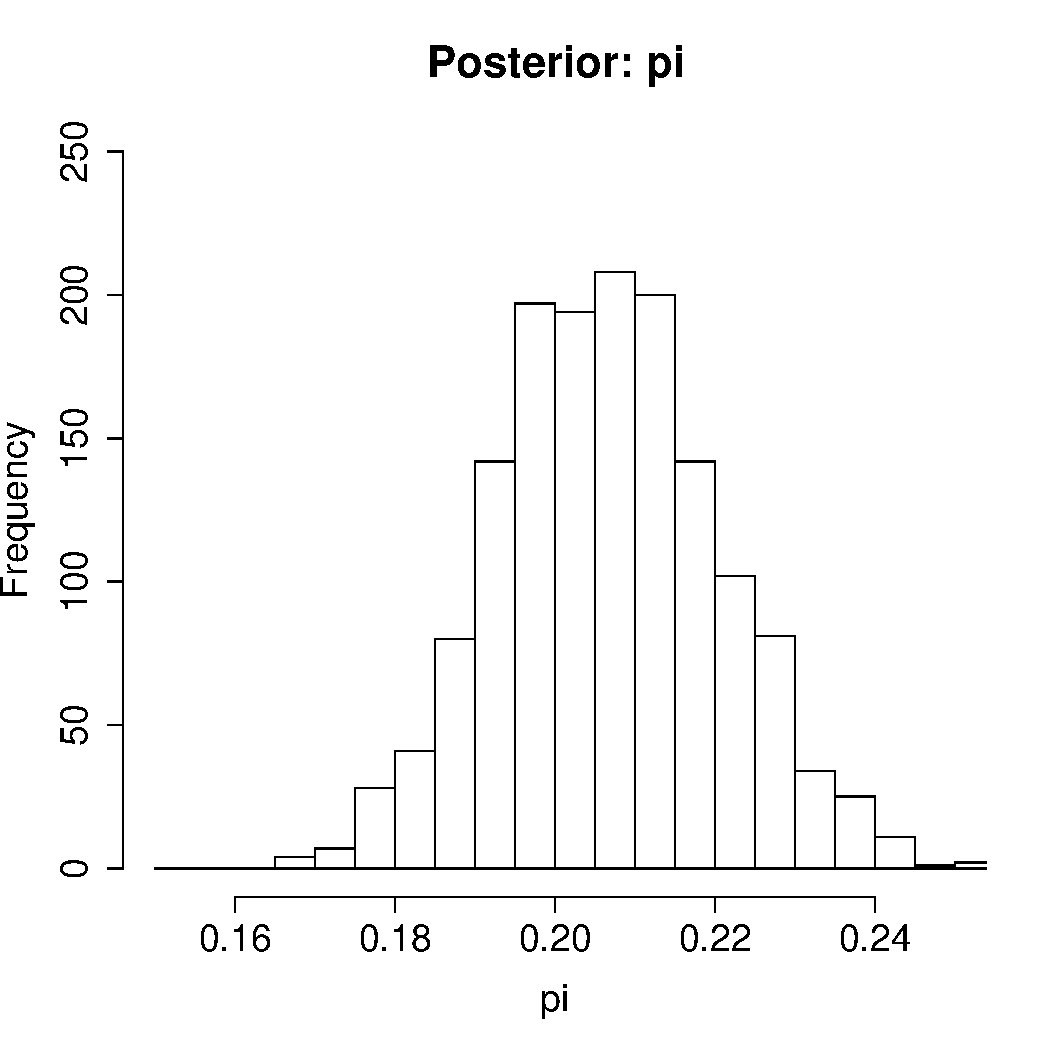
\includegraphics[width=0.35\textwidth]{pdf/beta-binomial-anno-posterior-pi.pdf}%

\sld{Sensitivity / Specificity Estimates}

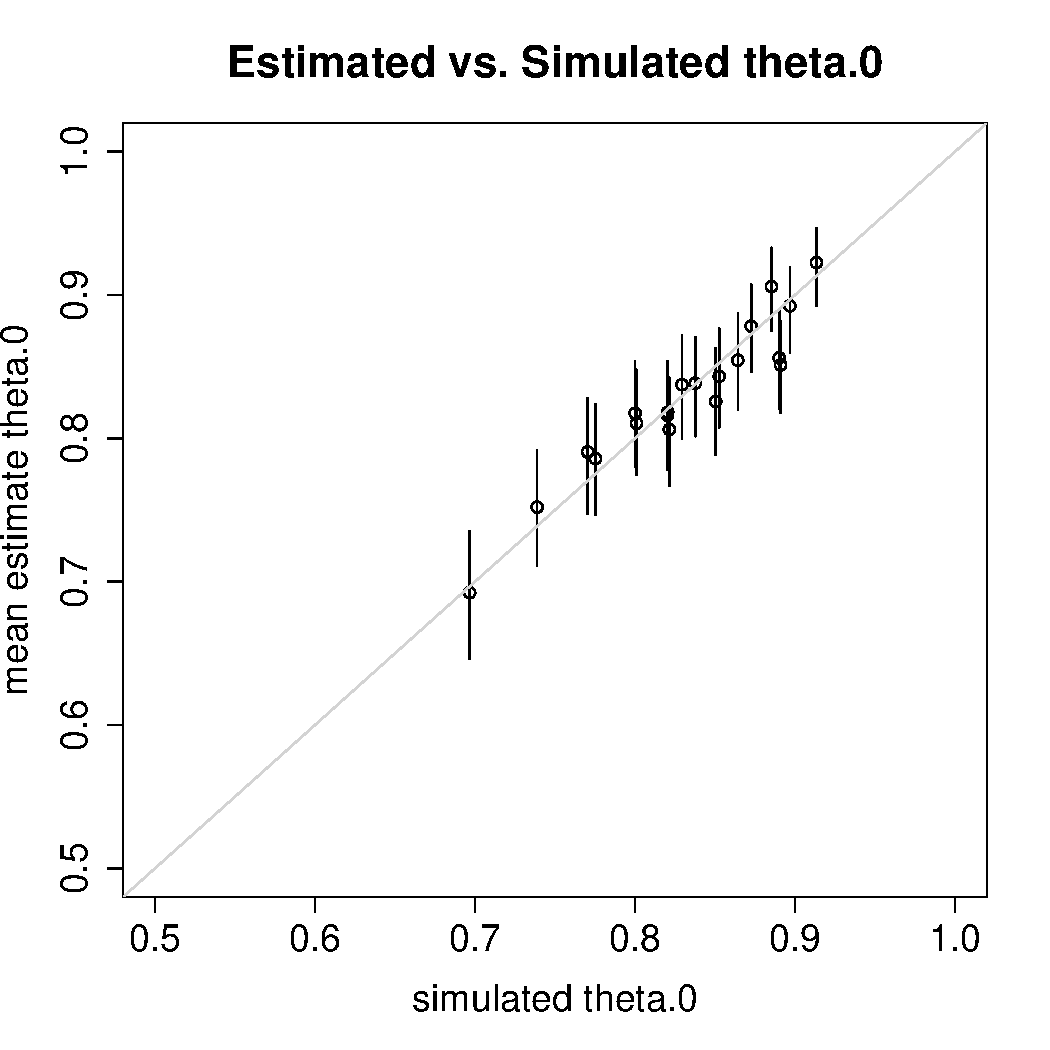
\includegraphics[width=0.4\textwidth]{pdf/beta-binomial-anno-theta0-fit.pdf}%
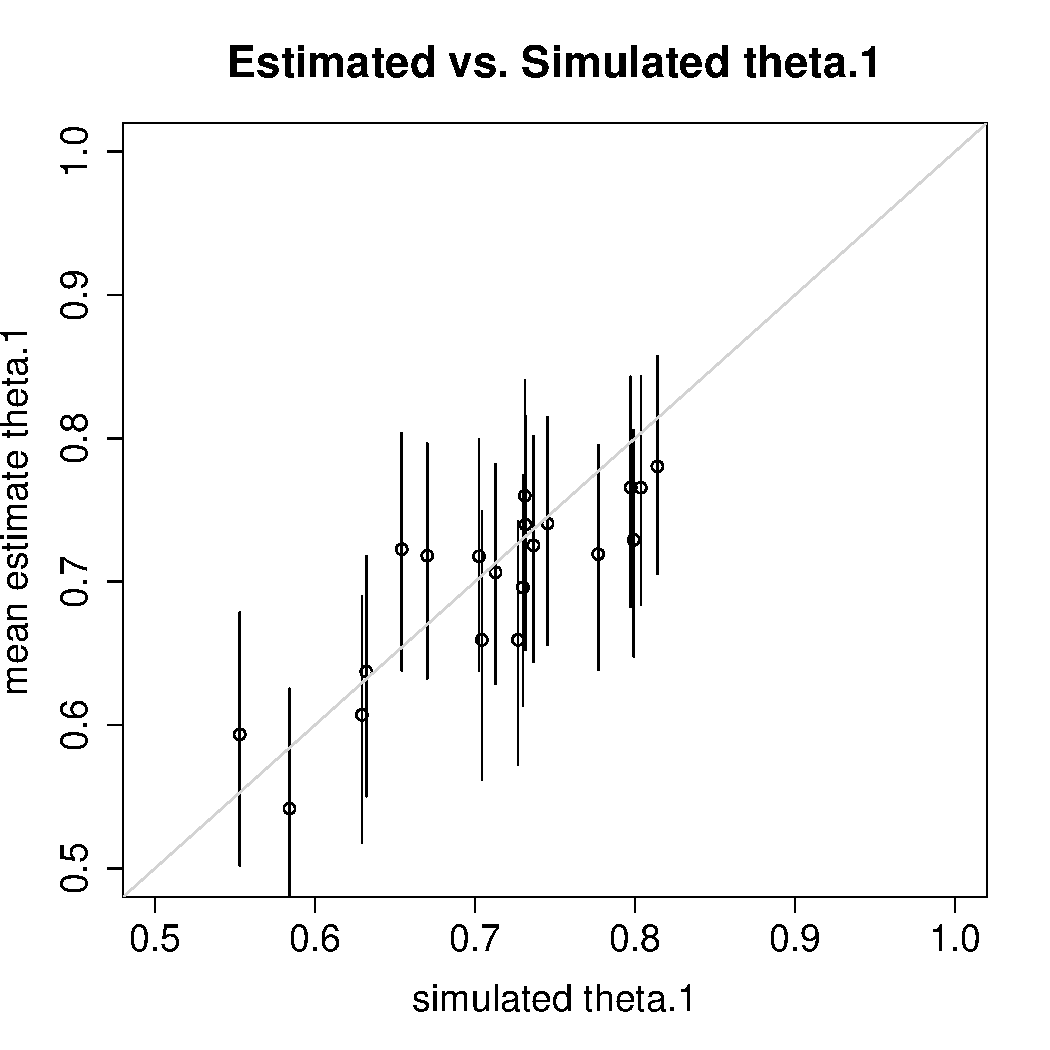
\includegraphics[width=0.4\textwidth]{pdf/beta-binomial-anno-theta1-fit.pdf}%
\vspace*{-12pt}
\begin{itemize}
\small
\item Posterior mean and 95\% intervals
\item Diagonal is perfect estimation
\item More uncertainty for sensitivity (more data w.\ $\pi = 0.2$)
\end{itemize}


\sld{Sens / Spec Hyperprior Estimates}

\noindent
{\small Posterior samples $\alpha^{(n)},\beta^{(n)}$; cross-hairs at known vals.}

\hspace*{-8pt}
\begin{tabular}{ll}
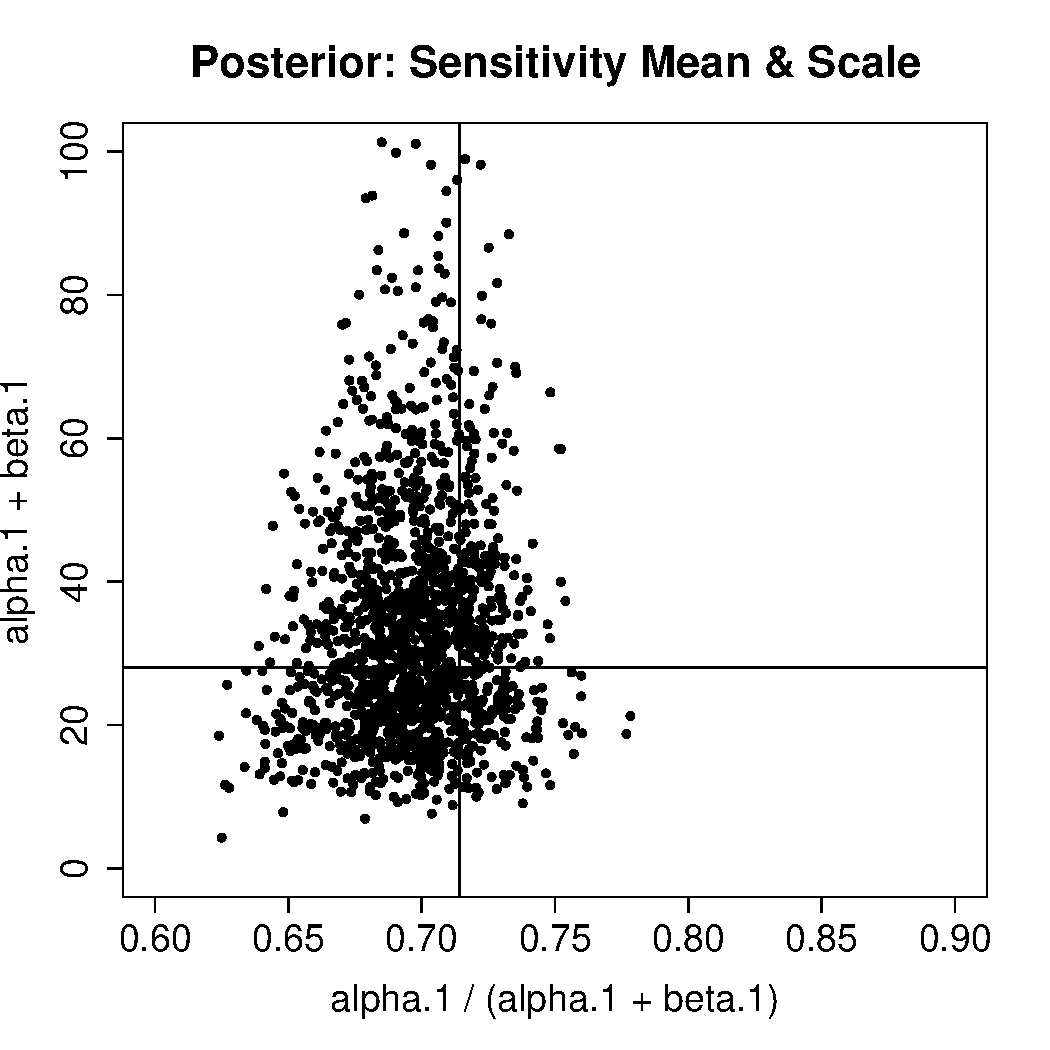
\includegraphics[width=0.40\textwidth]{pdf/beta-binomial-anno-scatter-sens.pdf}
&
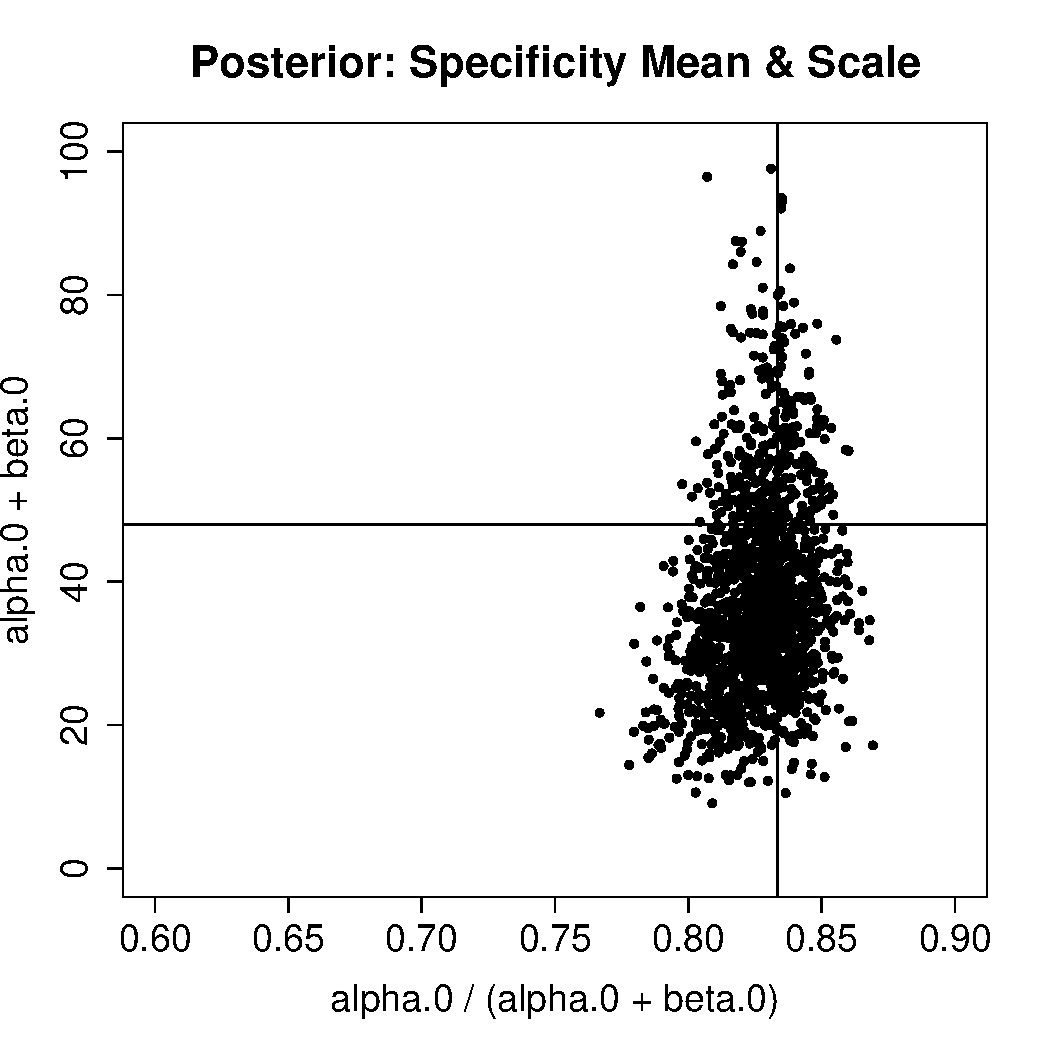
\includegraphics[width=0.40\textwidth]{pdf/beta-binomial-anno-scatter-spec.pdf}
\end{tabular}

\begin{itemize}
\item Note skew to high scale (low variance)
\item Estimates match sampled means
\end{itemize}


\newpage
\vspace*{36pt}
\noindent
{\huge Real Data}

\sld{5 Dentists Diagnosing Caries}

{\footnotesize
\begin{tabular}{cr|cr|cr}
{\it Dentists} & {\it Count} &
{\it Dentists} & {\it Count} &
{\it Dentists} & {\it Count}
\\ \hline
00000 & 1880 & 10000 & 22 & 00001 & 789 \\
10001 & 26 & 00010 & 43 & 10010 & 6 \\
00011 & 75 & 10011 & 14 & 00100 & 23 \\
10100 & 1 & 00101 & 63 & 10101 & 20 \\
00110 & 8 & 10110 & 2 & 00111 & 22 \\
10111 & 17 & 01000 & 188 & 11000 & 2 \\
01001 & 191 & 11001 & 20 & 01010 & 17 \\
11010 & 6 & 01011 & 67 & 11011 & 27 \\
01100 & 15 & 11100 & 3 & 01101 & 85 \\
11101 & 72 & 01110 & 8 & 11110 & 1 \\
01111 & 56 & 11111 & 100
\end{tabular}
}

\sld{Estimands of Interest}

\begin{itemize}
\item $\pi$: Prevalence of caries
\item $c_i$: 1 if patient $i$ has caries; 0 otherwise
\item $\theta_{1,j}$: Sensitivity of dentist $j$ \ \ \ {\small [ TP/(TP+FN) ]}
\item $\theta_{0,j}$: Specificity of dentist $j$ \ \ \ {\small [ TN/(TN+FP) ]}
\begin{itemize}
\footnotesize
\item can compute precision [ TP/(TP+FP) ]
\item precision + recall (sensitivity) not complete [no FN]
\end{itemize}
\vspace*{12pt}
\item task difficulty --- priors on $\theta$ predict new annotators
\item item difficulty
\end{itemize}


\sld{Posteriors for Dentist Accuracies}

\begin{itemize}
\item In beta-binomial by annotator model
\end{itemize}

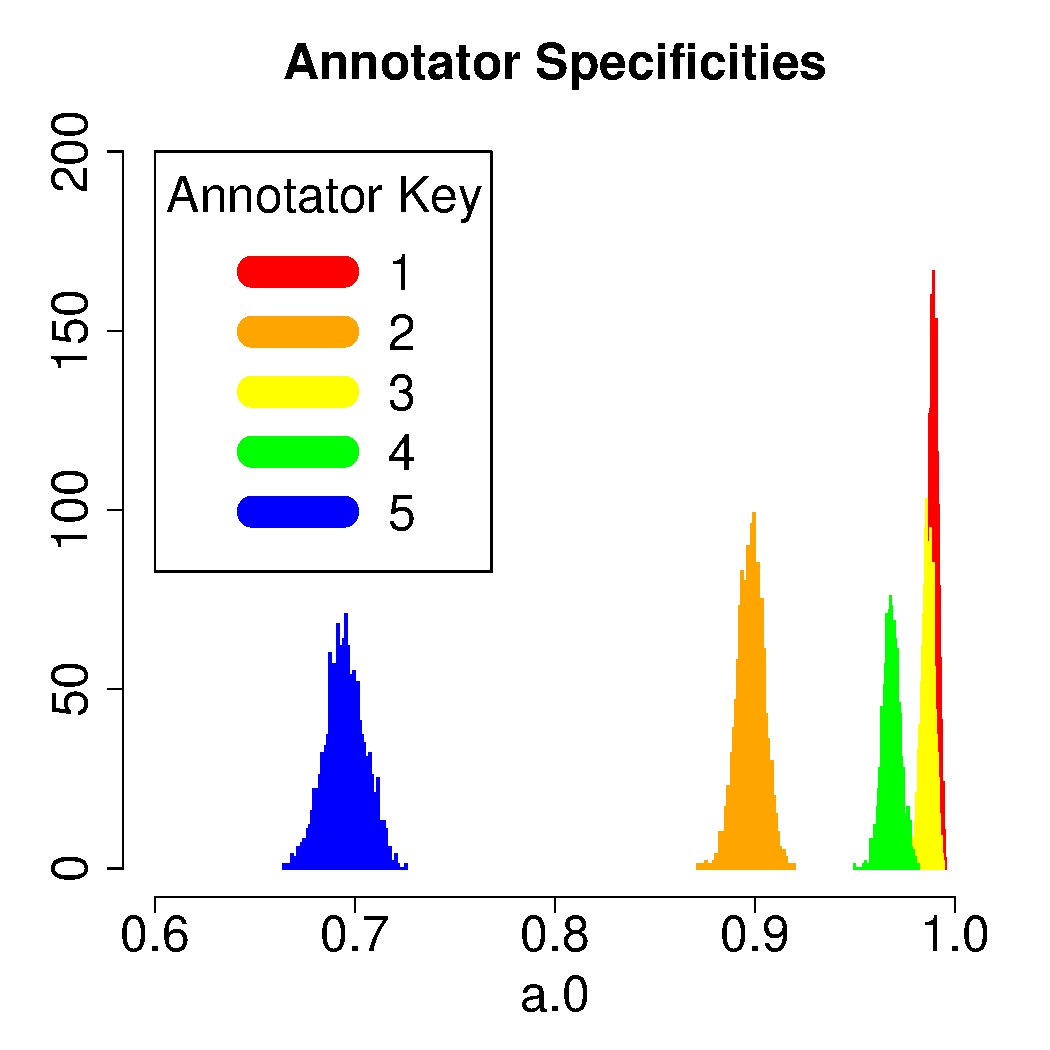
\includegraphics[width=0.4\textwidth]{pngs/a-0-hist.pdf}
\ \ \
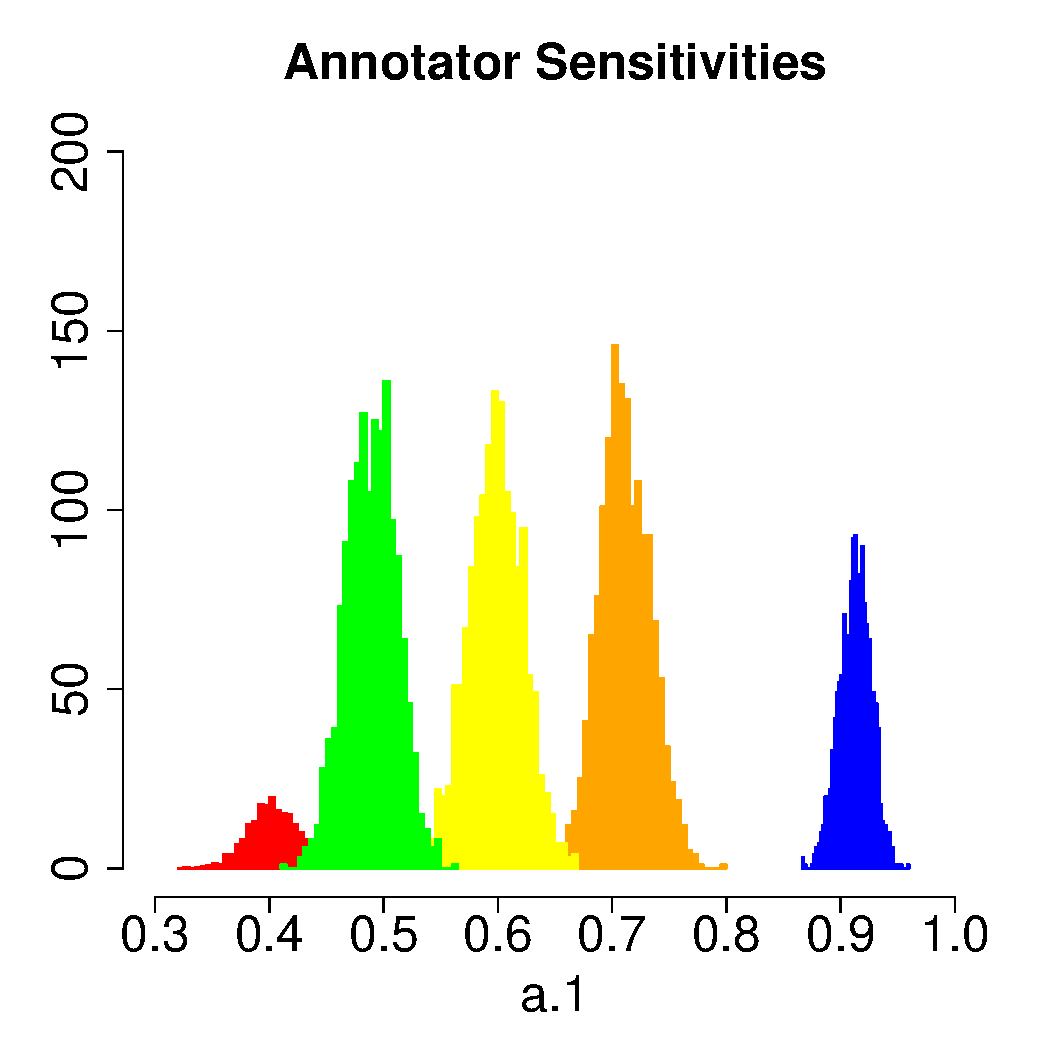
\includegraphics[width=0.4\textwidth]{pngs/a-1-hist.pdf}

\begin{itemize}
\item Posterior density vs. point estimates (e.g. mean)
\end{itemize}


\sld{Posteriors for Dentistry Data Items}

\hspace*{-24pt}
\begin{tabular}{ll}
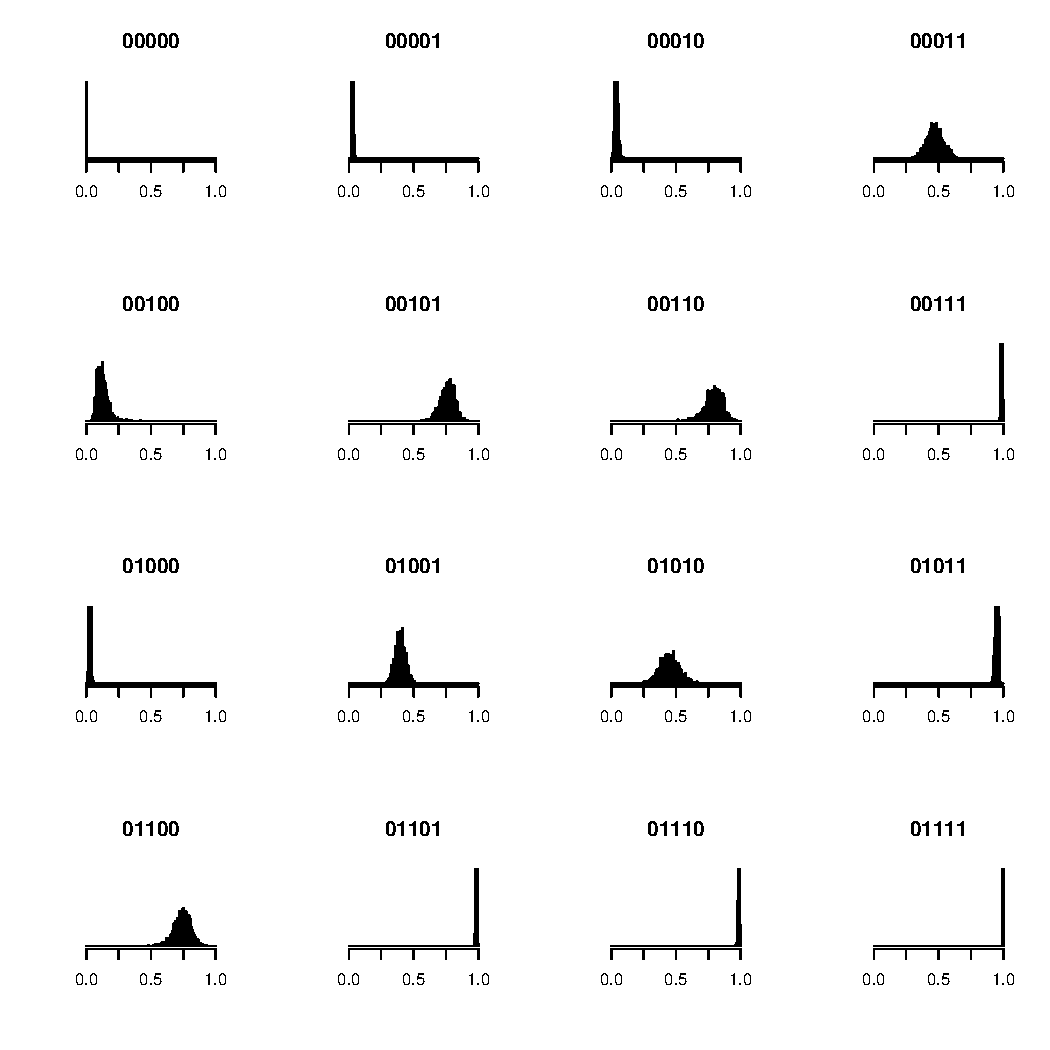
\includegraphics[width=0.5\textwidth]{pngs/model-4-cat-posteriors-dentistry.pdf}
&
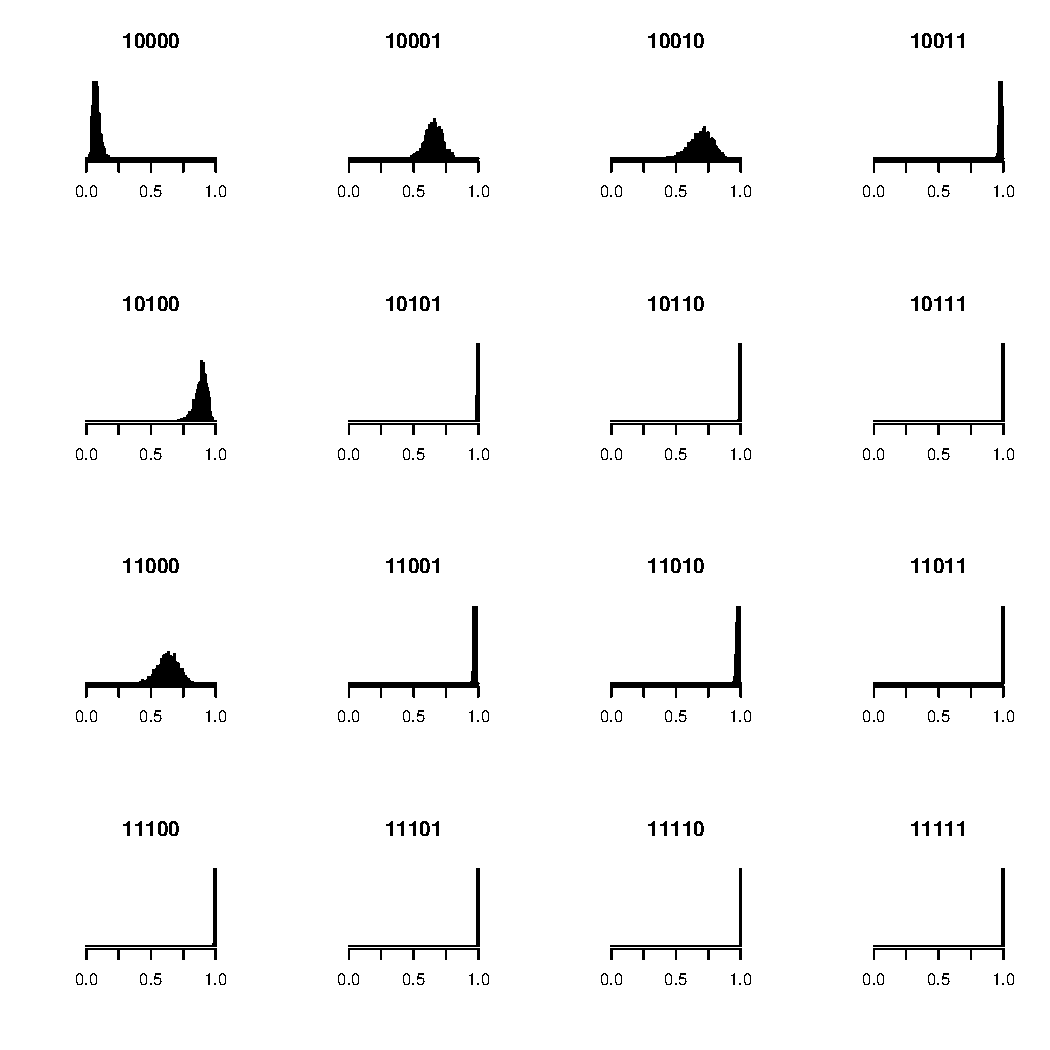
\includegraphics[width=0.5\textwidth]{pngs/model-4-cat-posteriors-dentistry-2.pdf}
\end{tabular}

Accounts for bias, so very different from simple vote!

\sld{Marginal Evaluation}

\begin{itemize}
\item Common eval in epidemiology
\item Models without sensitivity/specificity by annotator underdispersed
\end{itemize}

\begin{tabular}{rr|rrr}
{\it Positive} &   & \multicolumn{3}{c}{{\it Posterior Quantiles}} \\
{\it Tests} & {\it Frequency} & {\it .025} & {\it .5} & {\it .975} \\  \hline
0 & 1880 & 1818 & 1877 & 1935 \\
1 & 1065 & 1029 & 1068 & 1117 \\
2 & 404 & 385 & 408 & 434 \\
3 & 247 & 206 & 227 & 248 \\
4 & 173 & 175 & 193 & 212 \\
5 & 100 & 80 & 93 & 109 \\
\end{tabular}

\sld{Textual Entailment Data}

\begin{itemize}
\item Collected by Snow et al. using Mechnical Turk
\item Recreates a popular linguistic data set (Dagan et al.'s RTE-1)
\item {\it Text}: Microsoft was established in Italy in 1985.
\\ {\it Hypothesis}: Microsoft was established in 1985.
\item Binary responses true/false
\item ``Gold Standard'' was pretty bad
\end{itemize}

\sld{Estimated vs.\ ``Gold'' Accuracies}

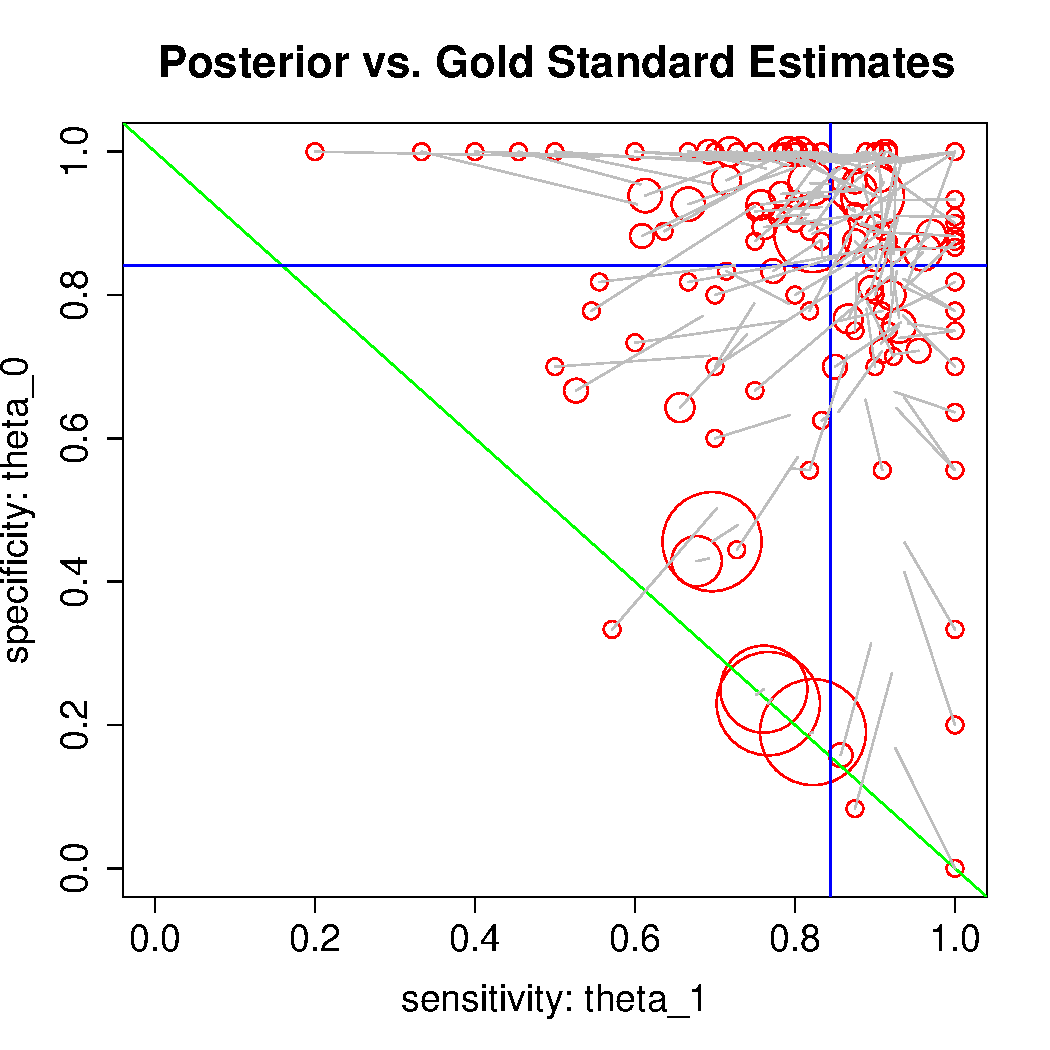
\includegraphics[width=0.4\textwidth]{pdf/dolores-rte-resids2D.pdf}%

\begin{itemize}\footnotesize
\item Diagonal green at chance (below is adversarial); blue lines at estimated prior means
\item Circle area is items annotated, center at ``gold standard'' accuracy, lines to estimated accuracy (note pull to prior)
\end{itemize}

\sld{Residual Category Errors}

\vspace*{-6pt}
\noindent
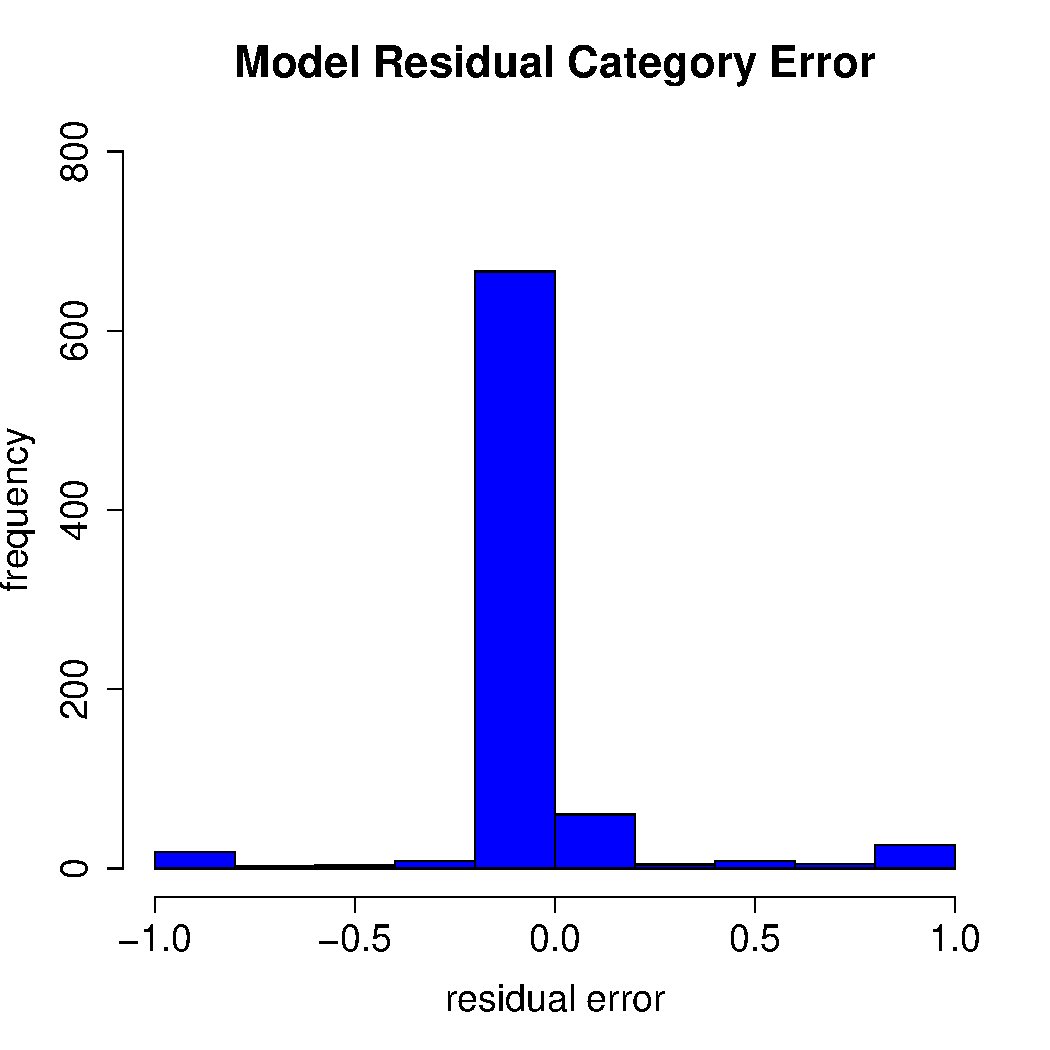
\includegraphics[width=0.3\textwidth]{pdf/dolores-cat-resids-model.pdf}%
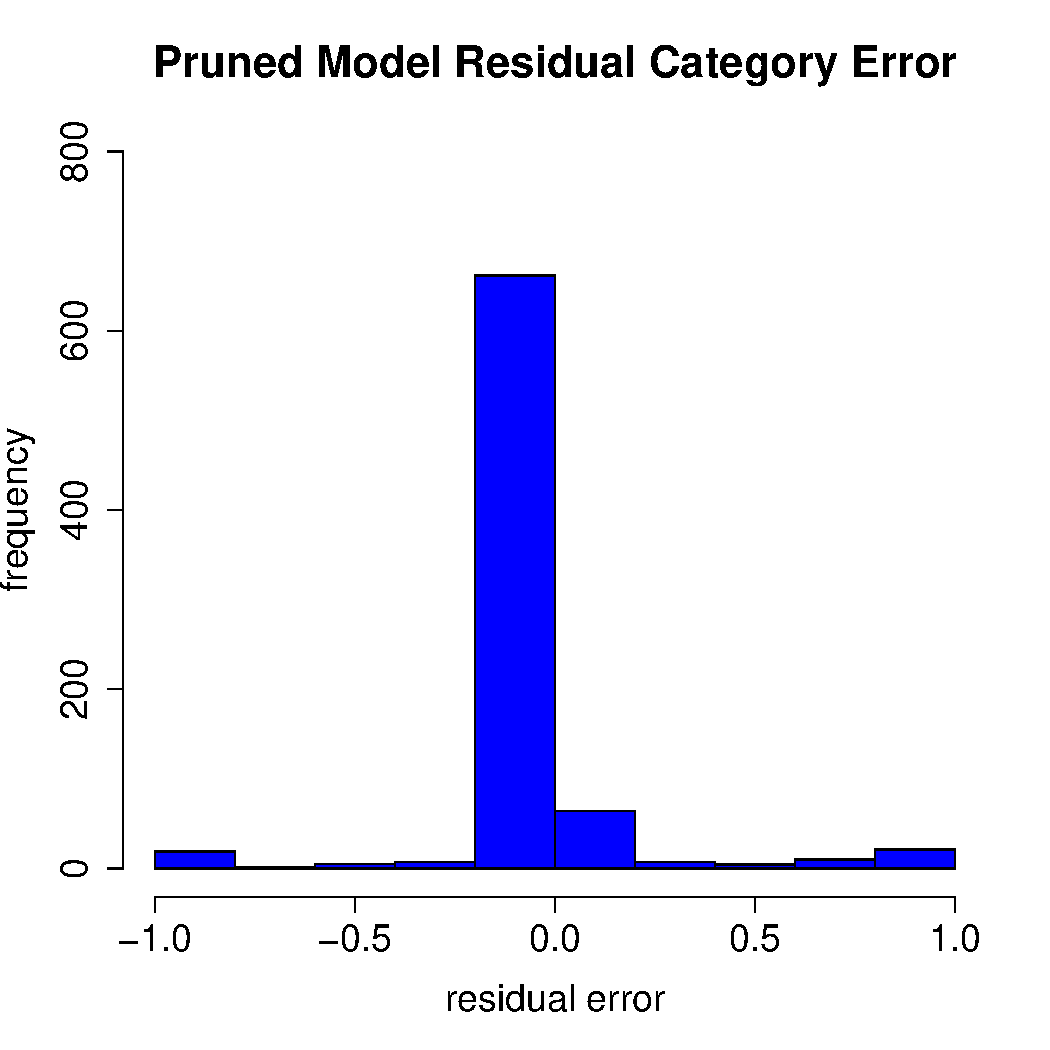
\includegraphics[width=0.3\textwidth]{pdf/dolores-cat-resids-model-pruned.pdf}%
\\[-2pt]
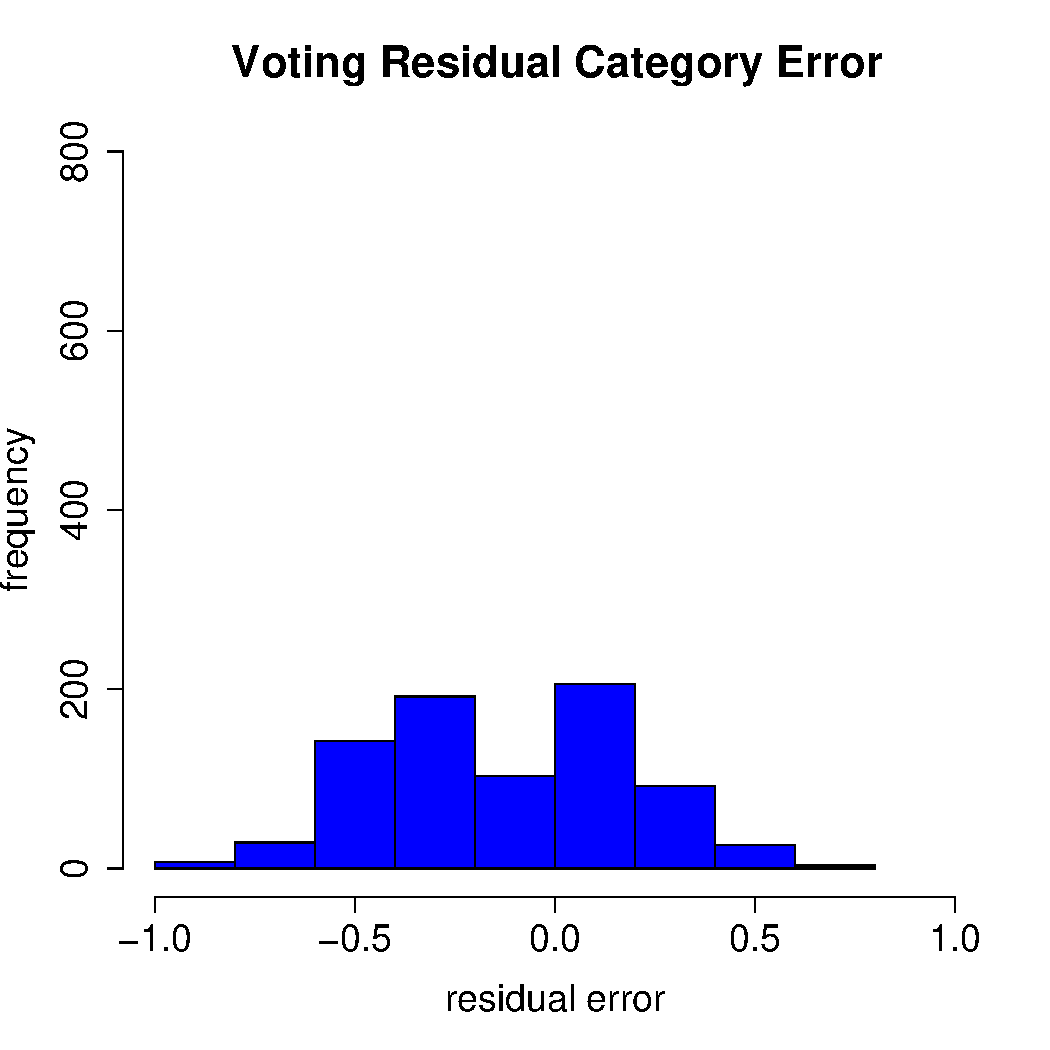
\includegraphics[width=0.3\textwidth]{pdf/dolores-cat-resids-voted.pdf}%
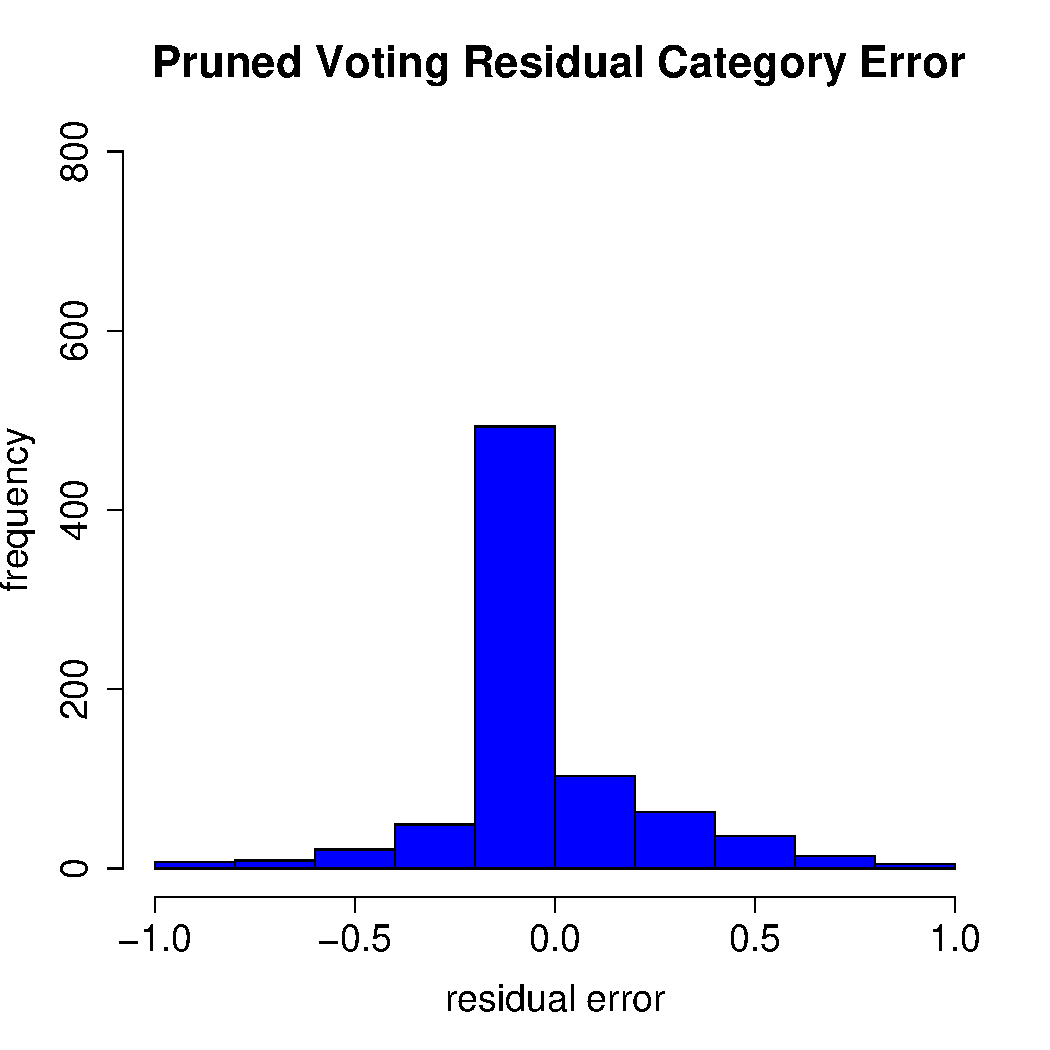
\includegraphics[width=0.3\textwidth]{pdf/dolores-cat-resids-voted-pruned.pdf}%
\vspace*{-8pt}
\begin{itemize}\footnotesize
\item Many residual errors in gold standard, not Turkers
\end{itemize}


\sld{Modeling Item Difficulty}

\begin{itemize}
\item Logistic Item-Response models with shape used in social sciences
(e.g. education and voting)
\item Use logistic scale (maps $(-\infty,\infty)$ to $[0,1]$)
\item $\alpha_j$: annotator $j$'s bias (ideally 0)
\item $\delta_j$: annotator $j$'s discriminativeness (ideally $\infty$)
\item $\beta_i$: item $i$'s ``location'' plus ``difficulty''
\item $x_i \sim \mbox{logit}^{-1}(\delta_j(\alpha_i - \beta_j))$
\end{itemize}

\sld{Modeling Item Difficulty (Cont.)}

\begin{itemize}
\item Place normal (or other) priors on coefficients,
\\[4pt]
e.g. \ $\beta_i \sim \mathsf{Norm}(0,\sigma^2)$, \ \ \ $\sigma^2 \sim \mathsf{Unif}(0,100)$
\item
Priors may be estimated as before; leads to pooling of item difficulties.
\item Need more than 5-10 coders/item for tight posterior on difficulties
\item Model has better $\chi^2$ fits, but many more params
\item Harder to estimate computationally in BUGS
\item Full details and code in paper
\end{itemize}


\sld{Extending Coding Types}

\begin{itemize}
\item Multinomial responses (Dirichlet-multinomial)
\item Ordinal responses (ordinal logistic model)
\item Scalar responses (continuos responses)
\end{itemize}

\sld{Probabilistic Training and Testing}

\begin{itemize}
\item Use probabilistic item posteriors for training
\item Use probabilistic item posteriors for testing
\item Directly with most probabilistic models (e.g. logistic regression, multinomial)
\item Or, train/test with posterior samples
\item Penalizes overconfidence of estimators (in log loss)
\item Demonstrated theoretical effectiveness (Smyth et al.)
\item Need to test in practice
\end{itemize}

\sld{The End}

\begin{itemize}
\item References
\begin{itemize}
\item {\tt http://lingpipe-blog.com/}
\end{itemize}
\item Contact
\begin{itemize}
\item
{\tt carp@alias-i.com}
\end{itemize}
\item
R/BUGS (Anon) Subversion Repository
\\[4pt]
{\tt\footnotesize svn co https://aliasi.devguard.com/svn/sandbox/hierAnno}
\end{itemize}

\end{document}

